\let\negmedspace\undefined
\let\negthickspace\undefined
\documentclass[journal]{IEEEtran}
\usepackage[a5paper, margin=10mm, onecolumn]{geometry}
%\usepackage{lmodern} % Ensure lmodern is loaded for pdflatex
\usepackage{tfrupee} % Include tfrupee package

\setlength{\headheight}{1cm} % Set the height of the header box
\setlength{\headsep}{0mm}     % Set the distance between the header box and the top of the text

\usepackage{gvv-book}
\usepackage{gvv}
\usepackage{cite}
\usepackage{amsmath,amssymb,amsfonts,amsthm}
\usepackage{algorithmic}
\usepackage{graphicx}
\usepackage{textcomp}
\usepackage{xcolor}
\usepackage{txfonts}
\usepackage{listings}
\usepackage{enumitem}
\usepackage{mathtools}
\usepackage{gensymb}
\usepackage{comment}
\usepackage[breaklinks=true]{hyperref}
\usepackage{tkz-euclide} 
\usepackage{listings}
% \usepackage{gvv}                                        
\def\inputGnumericTable{}                                 
\usepackage[latin1]{inputenc}                                
\usepackage{color}                                            
\usepackage{array}                                            
\usepackage{longtable}                                       
\usepackage{calc}                                             
\usepackage{multirow}                                         
\usepackage{hhline}                                           
\usepackage{ifthen}
\usepackage{lscape}
\begin{document}

\bibliographystyle{IEEEtran}



\title{2.10.54}
\author{EE25BTECH11057 - Rushil Shanmukha Srinivas
}
% \maketitle
% \newpage
% \bigskip
{\let\newpage\relax\maketitle}

\renewcommand{\thefigure}{\theenumi}
\renewcommand{\thetable}{\theenumi}
\setlength{\intextsep}{10pt} % Space between text and floats

\numberwithin{equation}{enumi}
\numberwithin{figure}{enumi}
\renewcommand{\thetable}{\theenumi}

\textbf{Problem:} Let $\vec{a},\vec{b},\vec{c} $ be unit vectors such that $\vec{a}+\vec{b}+\vec{c} = \vec{0} $ .Which of the following are correct?
\begin{enumerate}
\item $ \vec{a}\times\vec{b} = \vec{b}\times\vec{c} = \vec{c}\times\vec{a} = \vec{0} $
\item $ \vec{a}\times\vec{b} = \vec{b}\times\vec{c} = \vec{c}\times\vec{a} \neq \vec{0} $
\item $ \vec{a}\times\vec{b} = \vec{b}\times\vec{c} = \vec{a}\times\vec{c} \neq \vec{0} $
\item $ \vec{a}\times\vec{b},\vec{b}\times\vec{c},\vec{c}\times\vec{a} $ are mutually perpendicular.
\end{enumerate}
\textbf{Solution:}
Given ,
\begin{align}
\vec{a}+\vec{b}+\vec{c} = \vec{0} , \norm{\vec{a}} = \norm{\vec{b}} = \norm{\vec{c}} = 1
\end{align}
\begin{align}
(\vec{a}+\vec{b}+\vec{c})^2 = 0
\end{align}
\begin{align}
{\norm{\vec{a}}}^2+{\norm{\vec{b}}}^2+{\norm{\vec{c}}}^2+2\vec{a}^\top\vec{b}+2\vec{b}^\top\vec{c}+2\vec{c}^\top\vec{a} = 0
\end{align}
\begin{align}
\vec{a}^\top\vec{b}+\vec{b}^\top\vec{c}+\vec{c}^\top\vec{a} = \frac{-3}{2}
\end{align}
\begin{align}
\vec{a}+\vec{b}+\vec{c}=\vec{0} \Longrightarrow \myvec{\vec{a} & \vec{b} & \vec{c}}\myvec{1 \\1\\1} = \vec{0} \Longrightarrow
\vec{A}\vec{x} = \vec{0} 
\end{align}
\begin{align}
\vec{A}^\top\vec{A}\vec{x} = \vec{0} \Longrightarrow G\vec{x}=\vec{0}
\end{align}
\begin{align}
\myvec{
\norm{\vec{a}}^2 & \vec{a}^\top\vec{b} & \vec{c}^\top\vec{a} \\
\vec{a}^\top\vec{b} & \norm{\vec{b}}^2 & \vec{b}^\top\vec{c} \\
\vec{c}^\top\vec{a} & \vec{b}^\top\vec{c} & \norm{\vec{c}}^2 }
\myvec{
1 \\ 1 \\ 1} = \vec{0}
\end{align}
\begin{align}
\myvec{
1+\vec{a}^\top\vec{b}+\vec{c}^\top\vec{a} \\
\vec{a}^\top\vec{b}+1+\vec{b}^\top\vec{c} \\
\vec{c}^\top\vec{a}+\vec{b}^\top\vec{c}+1} = \myvec{0 \\ 0 \\ 0}
\end{align}
\begin{align}
1+\vec{a}^\top\vec{b}+\vec{c}^\top\vec{a} = \vec{a}^\top\vec{b}+1+\vec{b}^\top\vec{c} = 
\vec{c}^\top\vec{a}+\vec{b}^\top\vec{c}+1
\end{align}
\begin{align}
\vec{a}^\top\vec{b} = \vec{b}^\top\vec{c} = \vec{c}^\top\vec{a} 
\end{align}
From (4.4)
\begin{align}
\vec{a}^\top\vec{b} = \vec{b}^\top\vec{c} = \vec{c}^\top\vec{a} = \frac{-1}{2}
\end{align}
If
\begin{align}
\vec{a}^\top\vec{b} = \vec{b}^\top\vec{c} = \vec{c}^\top\vec{a} \Longrightarrow \vec{a}\times\vec{b} = \vec{b}\times\vec{c} = \vec{c}\times\vec{a}
\end{align}
\begin{align}
\vec{a}\times\vec{b} = \vec{b}\times\vec{c} = \vec{c}\times\vec{a} \neq \vec{0}
\end{align}

\begin{figure}[h!]
\centering
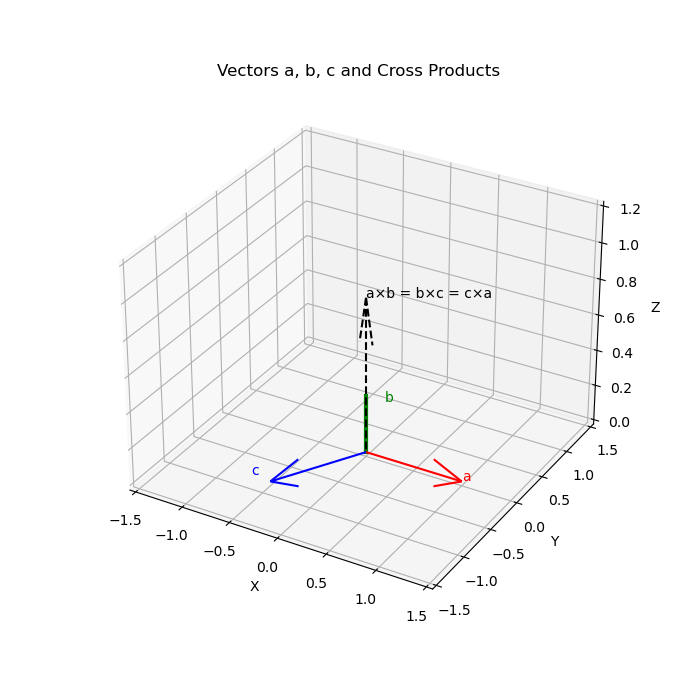
\includegraphics[width=0.9\columnwidth]{figs/figb.png} 
\caption*{Fig: Representation of vectors}
\label{Fig8}
\end{figure}

\end{document}